\section{\K 整流电路}

\Par 整流电路的种类较多,按交流电源的相数可分为单相和多相整流电路;按流过负载的电流波形可分为半波和全波整流电路.

\Par 我们只介绍单相整流电路.对于单相半波整流电路,我们很容易明白它的原理.
\begin{figure}[htbp]
	\centering
	\begin{minipage}[b]{0.48\textwidth}
        \centering
        \includegraphics[width=0.85\textwidth]{单相半波整流电路.pdf}
        \caption{单相半波整流电路}
        \label{fig:单相半波整流电路}
    \end{minipage}
    \begin{minipage}[b]{0.48\textwidth}
        \centering
        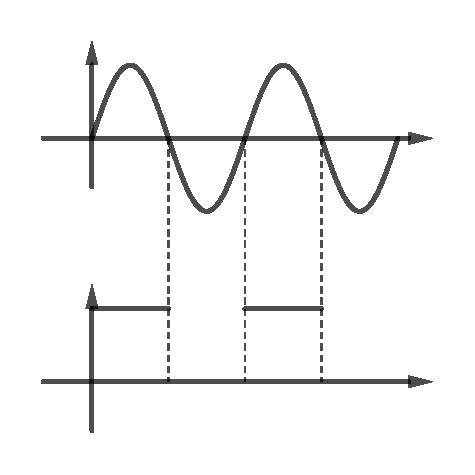
\includegraphics[width=0.85\textwidth]{单相半波整流电路特性曲线.pdf}
        \caption{单相半波整流电路特性曲线}
        \label{fig:单相半波整流电路特性曲线}
    \end{minipage}
\end{figure}

\Par 下面重点说明单相全波整流电路,由于画图困难,隧只在一张图上讲解.如图\ref{fig:单相桥式整流电路}所示,当输入的电压是上正下负的时候,可以知道$D_1$与$D_4$相交的节点是电位最高点,而$D_2$与$D_3$相交的节点是电位最低点,因此二极管$D_1$导通,视为导线.此时,$D_2$上端为高点位,下端为低电位,因此它截止.同理,$D_4$也将截止,而$D_3$导通.从而形成了电流依次流经$D_1$、$R_L$和$D_3$的电路,此时$R_L$上正下负.

\begin{figure}[htbp]
	\centering
	\includegraphics[width=0.65\textwidth]{单相桥式整流电路.jpg}
	\caption{单相桥式整流电路}
	\label{fig:单相桥式整流电路}
\end{figure}

\Par 同理,对于下正上负的输入电压有同样的分析,此时,$D_2$和$D_4$导通,$D_1$和$D_3$截止,从而形成了电流依次流经$D_2$、$R_L$和$D_4$的电路,$R_L$同样上正下负.

\Par 为了了解输出的整流电压的性质,我们需要知道整流电压的参数(设输入电压为$u=\sqrt{2}U_2\sin \omega t$):
\begin{enumerate}[(1)]
    \item 整流电压平均值$U_o$
    \begin{equation}
        U_o=\frac{2}{T}\int_0^{T/2}{\sqrt{2}U_2\sin \omega t\mathrm{d}t}\approx 0.9U_2
    \end{equation}
    \item 整流电流平均值$I_o$
    \begin{equation}
        I_o=\frac{U_o}{R_L}=0.9\frac{U_2}{R_L}
    \end{equation}
    \item 每管电流平均值$I_D$
    \begin{equation}
        I_D=\frac{1}{2}I_o=0.45\frac{U_2}{R_L}
    \end{equation}
    \item 每管承受的最高反向电压$U_{DRM}$
    \begin{equation}
        U_{DRM}=\sqrt{2}U_2
    \end{equation}
    \item 变压器副边电流有效值$I_2$
    \begin{equation}
        I_o=\frac{2}{T}\int_0^{T/2}{\sqrt{2}I_2\sin \omega t\mathrm{d}t}\approx 0.9I_2\Longrightarrow I_2\approx 1.1I_o
    \end{equation}
\end{enumerate}

\Par 通常我们用一个整流桥(硅桥堆)来代替四个二极管拼成的单相桥式整流电路,它就相当于一个黑箱.



